%versi 3 (22-07-2020)
\chapter{Landasan Teori}
\label{chap:teori}

\section{\textit{Command Line}}
\label{sec:commandline}
\textit{Command line} (atau \cli) dapat diartikan sebagai tampilan antarmuka/\textit{interface} yang memproses perintah dari pengguna dan meneruskannya langsung ke sistem operasi untuk dijalankan. Seluruh sistem operasi komputer yang ada memiliki sebuah \cli dalam bentuk \textit{shell}, yang dapat digunakan oleh penggunanya untuk langsung mengakses fungsi atau servis yang disediakan oleh sistem operasi. Sedangkan, perangkat lunak yang memproses \cli ini disebut sebagai \cl \textit{interpreter}, atau \cl \textit{processor}.

%Untuk hampir seluruh distribusi dari sistem operasi Linux, perangkat lunak \textit{shell}-nya bernama \textit{bash}, yang merupakan singkatan dari ``\textbf{B}ourne \textbf{A}gain \textbf{Sh}ell''.\cite{shottsjr:2019:linuxcommandline}

\subsection{\textit{Command Line Interface} dan \textit{Graphical User Interface}}
\label{sec:commandline-comparison}

Ada beberapa dari tipe antarmuka yang masih banyak digunakan di zaman sekarang, tetapi dua tipe yang paling banyak muncul adalah \cli dan \gui. Perangkat lunak berbasis \cl sendiri bisa memiliki berbagai macam tampilan, tetapi semuanya selalu mengikuti satu bentuk antarmuka umum. Bentuk yang dimaksud adalah sebuah area/\textit{window} yang memuat teks berupa perintah-perintah dari user untuk dilakukan oleh komputer, beserta keluarannya yang juga berupa teks, seperti dapat dilihat pada gambar \ref{fig:commandline-cli}. Jenis perangkat lunak seperti ini disebut memiliki antarmuka jenis \cli (CLI). Adapun dekorasi visual yang dimiliki oleh jenis tampilan ini hanya berupa warna pada teks-teks yang ada, tanpa tambahan gambar apapun. Jika perangkat lunak tersebut memiliki dekorasi dan/atau tombol interaktif berupa gambar grafis, seperti pada gambar \ref{fig:commandline-gui}, maka perangkat lunak tersebut dikategorikan sebagai perangkat lunak berbasis \gui.

\begin{figure}[ht]
    \begin{subfigure}[b]{0.475\linewidth}
		\centering
		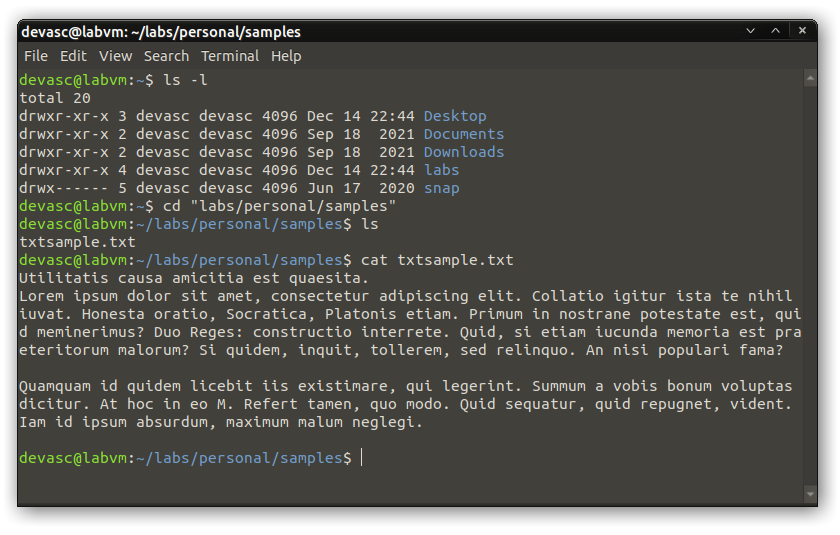
\includegraphics[height=4.7cm]{terminal-linux}
		\caption{Antarmuka perangkat lunak berbasis \cli.}
		\label{fig:commandline-cli}
	\end{subfigure}
	\hfill
    \begin{subfigure}[b]{0.475\linewidth}
		\centering
		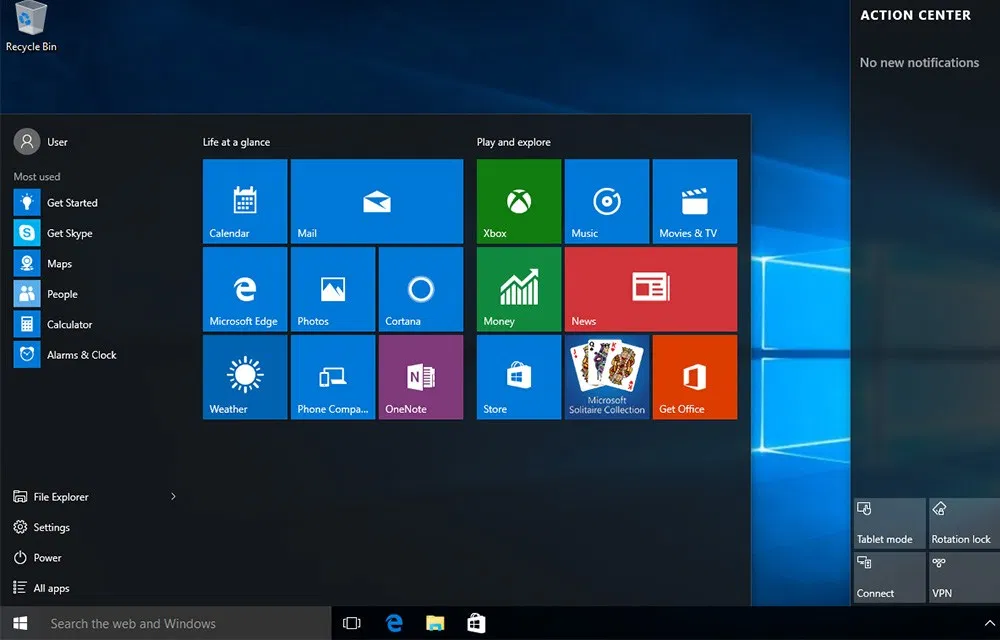
\includegraphics[height=4.5cm]{gui}
		\caption{Antarmuka perangkat lunak berbasis \gui.}
		\label{fig:commandline-gui}
	\end{subfigure}
    \caption[Dua jenis tampilan perangkat lunak]{Contoh dua jenis antarmuka (\textit{interface)} perangkat lunak.}
	\label{fig:commandline-interfacetypes}
\end{figure}

Selain dari tampilannya sendiri, ada beberapa perbedaan utama lain antara perangkat-perangkat lunak berbasis \cli dengan perangkat lunak berbasis \gui. Adapun perbedaan-perbedaan utama dari kedua jenis antarmuka ini adalah sebagai berikut.
\begin{itemize}
	\item Pengunaan sumber daya sistem untuk menjalankan perangkat lunak berbasis \cli lebih rendah dibandingkan dengan perangkat lunak berbasis \gui.
	\item Bagi pengguna pemula (atau pengguna awam pada umumnya), perangkat lunak berbasis \cli akan lebih sulit digunakan karena tidak adanya bantuan apapun dalam bentuk visual, sehingga satu-satunya cara untuk tahu bagaimana cara menggunakan fitur-fiturnya adalah melalui dokumentasi perangkat lunak yang ada. Karena alasan yang sama pula, perangkat lunak berbasis \cli lebih sulit untuk dibiasakan penggunaannya.
	\item Automasi perintah yang bersifat berulan-ulang jauh lebih mudah dilakukan pada perangkat lunak berbasis \cli. Hal ini dikarenakan perangkat lunak berbasis \cli tidak hanya lebih mudah untuk dibuat \textit{script}-nya, tetapi juga lebih efisien untuk digunakan ketika ada banyak sekali perintah yang harus dilakukan pada suatu saat tertentu.
\end{itemize}

\subsection{Cara Kerja \textit{Command Line}}
\label{sec:commandline-workings}

\subsection{Tipe \textit{Command Line}}
\label{sec:commandline-type}


\section{KIRI}
\label{sec:kiri}

\section{Skripsi}
\label{sec:skripsi} 
 
Rencananya akan diisi dengan penjelasan umum mengenai buku skripsi.

\dtext{11-12} 

\section{\LaTeX}
\label{sec:latex}

Mengapa menggunakan \LaTeX{} untuk buku skripsi dan apa keunggulan/kerugiannya bagi mahasiswa dan pembuat template. 

\dtext{13-14}


\section{Template Skripsi FTIS UNPAR}
\label{sec:template}
 
Akan dipaparkan bagaimana menggunakan template ini, termasuk petunjuk singkat membuat referensi, gambar dan tabel.
Juga hal-hal lain yang belum terpikir sampai saat ini. 
 
\dtext{15-16}

\subsection{Tabel}  
Berikut adalah contoh pembuatan tabel. 
Penempatan tabel dan gambar secara umum diatur secara otomatis oleh \LaTeX{}, perhatikan contoh di file bab2.tex untuk melihat bagaimana cara memaksa tabel ditempatkan sesuai keinginan kita.

Perhatikan bawa berbeda dengan penempatan judul gambar gambar, keterangan tabel harus diletakkan di atas tabel!!
Lihat Tabel~\ref{tab:contoh1} berikut ini:

\begin{table}[H] %atau h saja untuk "kira kira di sini"
	\centering 
	\caption{Tabel contoh}
	\label{tab:contoh1}
	\begin{tabular}{cccc}
		\toprule
		& $v_{start}$ & $\mathcal{S}_{1}$ & $v_{end}$\\

		\midrule
		$\tau_{1}$ & 1 & 12& 20\\
		$\tau_{2}$ & 1 &  & 20\\
		$\tau_{3}$ & 1 & 9 & 20\\
		$\tau_{4}$ & 1 &  & 20\\

		\bottomrule
		
	\end{tabular} 
\end{table}
Tabel~\ref{tab:cthwarna1} dan Tabel~\ref{tab:cthwarna2} berikut ini adalah tabel dengan sel yang berwarna dan ada dua tabel yang bersebelahan. 
\begin{table}[H]
	\begin{minipage}[c]{0.49\linewidth}
		\centering
		\caption{Tabel bewarna(1)}
		\label{tab:cthwarna1}
		\begin{tabular}{ccccc}
			\toprule
			 & $v_{start}$ & $\mathcal{S}_{2}$ & $\mathcal{S}_{1}$ & $v_{end}$\\
			
			\midrule
			$\tau_{1}$ & 1 & 5 \cellcolor{green}& 12& 20\\
			$\tau_{2}$ & 1 & 8 \cellcolor{green}& & 20\\
			$\tau_{3}$ & 1 & 2/8/17 \cellcolor{green}& 9 & 20\\
			$\tau_{4}$ & 1 & \cellcolor{red}& & 20\\
			
			\bottomrule

		\end{tabular}
	\end{minipage}
	\begin{minipage}[c]{0.49\linewidth}
		
		\centering 
		\caption{Tabel bewarna(2)}
		\label{tab:cthwarna2}
		\begin{tabular}{ccccc}
			\toprule
			 & $v_{start}$ & $\mathcal{S}_{1}$ & $\mathcal{S}_{2}$ & $v_{end}$\\
			
			\midrule
			$\tau_{1}$ & 1 & 12& 5 \cellcolor{red} &20\\
			$\tau_{2}$ & 1 &  &  8 \cellcolor{green} &20\\
			$\tau_{3}$ & 1 & 9 & 2/8/17 \cellcolor{green} &20\\
			$\tau_{4}$ & 1 &   & \cellcolor{red} &20\\
			
			\bottomrule
		
		\end{tabular}
	\end{minipage}
\end{table}

 
\subsection{Kutipan}
\label{subs:kutipan} 
Berikut contoh kutipan dari berbagai sumber, untuk keterangan lebih lengkap, silahkan membaca file referensi.bib yang disediakan juga di template ini.
Contoh kutipan:
\begin{itemize}
	\item Buku:~\cite{berg:08:compgeom} 
	\item Bab dalam buku:~\cite{kreveld:04:GIS}
	\item Artikel dari Jurnal:~\cite{buchin:13:median}
	\item Artikel dari prosiding seminar/konferensi:~\cite{kreveld:11:median}
	\item Skripsi/Thesis/Disertasi:~\cite{lionov:02:animasi}~\cite{wiratma:10:following}~\cite{wiratma:22:later}
	\item Technical/Scientific Report:~\cite{kreveld:07:watertight}
	\item RFC (Request For Comments):~\cite{RFC1654}
	\item Technical Documentation/Technical Manual:~\cite{Z.500}~\cite{unicode:16:stdv9}~\cite{google:16:and7}
	\item Paten:~\cite{webb:12:comm}
	\item Tidak dipublikasikan:~\cite{wiratma:09:median}~\cite{lionov:11:cpoly}
	\item Laman web:~\cite{erickson:03:cgmodel}  
	\item Lain-lain:~\cite{agung:12:tango}
\end{itemize}    
  
\subsection{Gambar}

Pada hampir semua editor, penempatan gambar di dalam dokumen \LaTeX{} tidak dapat dilakukan melalui proses {\it drag and drop}.
Perhatikan contoh pada file bab2.tex untuk melihat bagaimana cara menempatkan gambar.
Beberapa hal yang harus diperhatikan pada saat menempatkan gambar:
\begin{itemize}
	\item Setiap gambar {\bf harus} diacu di dalam teks (gunakan {\it field} {\sc label})
	\item {\it Field} {\sc caption} digunakan untuk teks pengantar pada gambar. Terdapat dua bagian yaitu yang ada di antara tanda $[$ dan $]$ dan yang ada di antara tanda $\{$ dan $\}$. Yang pertama akan muncul di Daftar Gambar, sedangkan yang kedua akan muncul di teks pengantar gambar. Untuk skripsi ini, samakan isi keduanya.
	\item Jenis file yang dapat digunakan sebagai gambar cukup banyak, tetapi yang paling populer adalah tipe {\sc png} (lihat Gambar~\ref{fig:ularpng}), tipe {\sc jpg} (Gambar~\ref{fig:ularjpg}) dan tipe {\sc pdf} (Gambar~\ref{fig:ularpdf})
	\item Besarnya gambar dapat diatur dengan {\it field} {\sc scale}.
	\item Penempatan gambar diatur menggunakan {\it placement specifier} (di antara tanda  $[$ dan $]$ setelah deklarasi gambar.
	Yang umum digunakan adalah {\bf H} untuk menempatkan gambar {\bf sesuai} penempatannya di file .tex atau  {\bf h} yang berarti "kira-kira" di sini. \\
	Jika tidak menggunakan {\it placement specifier}, \LaTeX{} akan menempatkan gambar secara otomatis untuk menghindari bagian kosong pada dokumen anda.
	Walaupun cara ini sangat mudah, hindarkan terjadinya penempatan dua gambar secara berurutan. 	
	\begin{itemize}
		\item Gambar~\ref{fig:ularpng} ditempatkan di bagian atas halaman, walaupun penempatannya dilakukan setelah penulisan 3 paragraf setelah penjelasan ini.
		\item Gambar~\ref{fig:ularjpg} dengan skala 0.5 ditempatkan di antara dua buah paragraf. Perhatikan penulisannya di dalam file bab2.tex!
		\item Gambar~\ref{fig:ularpdf} ditempatkan menggunakan {\it specifier} {\bf h}.
	\end{itemize}
\end{itemize}
 
\dtext{17-18}
\begin{figure} 
	\centering  
	\includegraphics[scale=1]{ular-png}  
	\caption[Gambar {\it Serpentes} dalam format png]{Gambar {\it Serpentes} dalam format png} 
	\label{fig:ularpng} 
\end{figure} 

\dtext{19-20}
\begin{figure}[H]
	\centering  
	\includegraphics[scale=0.5]{ular-jpg}  
	\caption[Ular kecil]{Ular kecil} 
	\label{fig:ularjpg} 
\end{figure} 
\dtext{21-22}

\begin{figure}[ht] 
	\centering  
	\includegraphics[scale=1]{ular-pdf}  
	\caption[ {\it Serpentes} betina]{ {\it Serpentes} jantan} 
	\label{fig:ularpdf} 
\end{figure} 
 
\subsection{Kode Program}

Kode program dalam bahasa tertentu seringkali harus ditulis di dalam bab, bukan hanya dilampirkan di bagian Lampiran. 
Kode~\ref{kode:aneh} menampilkan penggunaan karakter-karakter yang umum digunakan dalam sebuah program yang ditulis dengan bahasa C.


\begin{lstlisting}[language=Java, caption=Kode untuk menampilkan karakter-karakter aneh, label=kode:aneh]
// This does not make algorithmic sense, 
// but it shows off significant programming characters.

#include<stdio.h>

void myFunction( int input, float* output ) {
	switch ( array[i] ) {
		case 1: // This is silly code
			if ( a >= 0 || b <= 3 && c != x )
				*output += 0.005 + 20050;
			char = 'g';
			b = 2^n + ~right_size - leftSize * MAX_SIZE;
			c = (--aaa + &daa) / (bbb++ - ccc % 2 );
			strcpy(a,"hello $@?"); 
	}
	count = ~mask | 0x00FF00AA;
}

// Fonts for Displaying Program Code in LATEX
// Adrian P. Robson, nepsweb.co.uk
// 8 October 2012
// http://nepsweb.co.uk/docs/progfonts.pdf

\end{lstlisting}

\subsection{Notasi}

Simbol-simbol (matematika) yang sering digunakan sepanjang penulisan skripsi, dapat dimasukkan ke dalam ``Daftar Notasi''. Daftar ini ada di halaman depan sebelum Bab~\ref{chap:intro}.
Cara memasukkan sebuah simbol ke dalam Daftar Notasi adalah menggunakan perintah \verb|\nomenclature|. Contoh:
\begin{center}
    \verb|\nomenclature[]{$A$}{luas kandang ular}|    
\end{center}
\nomenclature[]{$A$}{luas kandang ular}
\nomenclature[]{$n$}{banyaknya ular}
\nomenclature[]{$k$}{jumlah kepala per seekor ular\nomrefpage}
Argumen opsional digunakan untuk mengurutkan notasi. Silahkan lihat sendiri dokumentasi package \verb|nomencl|

